\documentclass[a4paper,12pt]{article}
%宏包
\usepackage{amsmath}
\usepackage{amssymb}
\usepackage{amsthm}
\usepackage{geometry}
\usepackage{natbib}%bibtex
\usepackage[dvipsnames]{xcolor}
\usepackage{tcolorbox}
\usepackage{enumerate}
\usepackage{tikz}
\usepackage{float}
\usepackage{caption}
\usepackage[colorlinks,linkcolor=cyan!40!black]{hyperref}
\usepackage{enumerate}
\usepackage{xeCJK}
\setCJKmainfont{SimSun}

%页面设置
\linespread{1.1}
\geometry{a4paper,left=2cm,right=2cm,top=2.5cm,bottom=2cm}

%环境和宏指令
\newenvironment{prooff}{{\noindent\it\textcolor{cyan!40!black}{Proof}:}\quad}{\par}
\newcommand{\bbrace}[1]{\left\{ #1 \right\} }
\newcommand{\bb}[1]{\mathbb{#1}}
\newcommand{\p}{^{\prime}}
\renewcommand{\mod}[1]{(\text{mod}\,#1)}
%ctrl+点击文本返回代码  选中代码 ctrl+alt+j 为代码查找文本


%定理环境
\newtheorem{defn}{Definition}
\newtheorem{coro}[defn]{Corollary}
\newtheorem{theo}[defn]{Theorem}
\newtheorem{exer}[defn]{Exercise}
\newtheorem{rema}[defn]{Remark}
\newtheorem{lem}[defn]{Lemma}
\newtheorem{prop}[defn]{Proposition}
\newtheorem{ques}{Question}

\title{Curriculum Vitae}
\date{}
\author{}

\begin{document}
\maketitle
\begin{minipage}{0.65\textwidth}
    \noindent\textbf{Name:} Erzhuo Wang(王尔卓) \\
    \textbf{Email:} wez2003211@gmail.com\\
    \textbf{Homepage:} \url{https://wez2003.github.io}
\end{minipage}
\begin{minipage}{0.13\textwidth}
    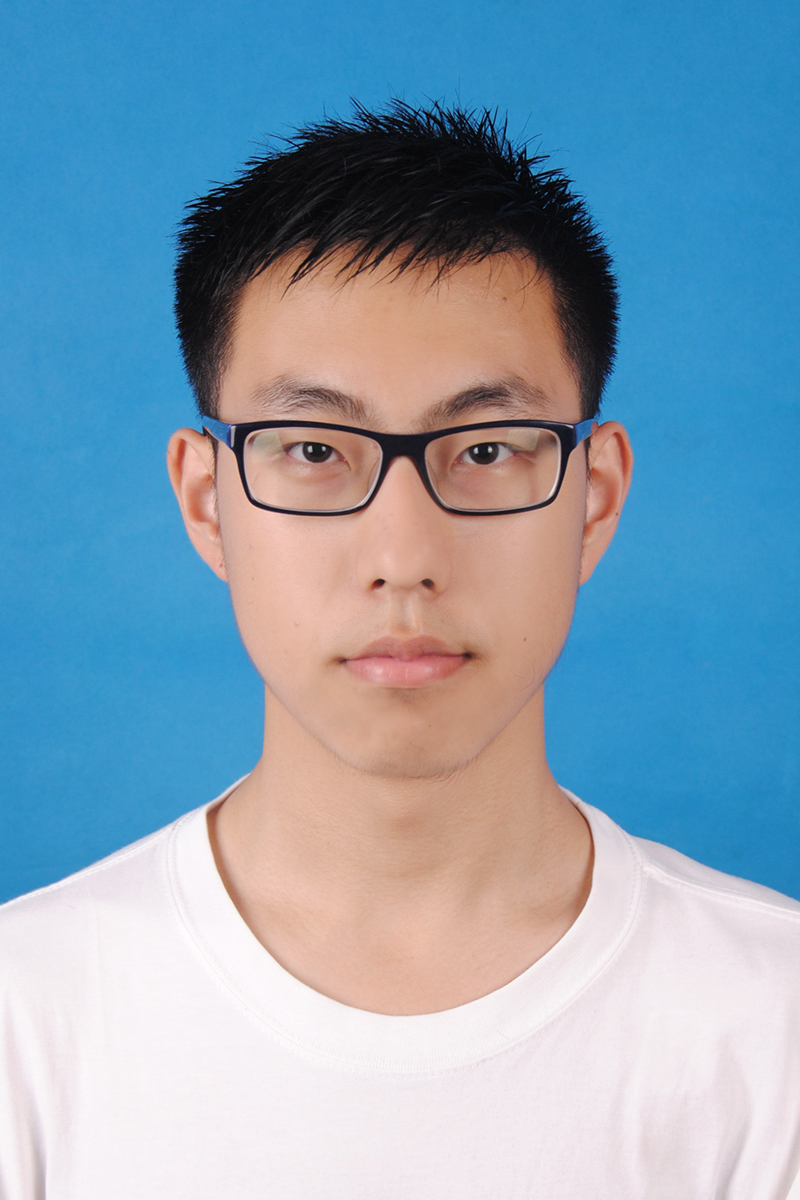
\includegraphics[width=\textwidth]{blue.jpg}
\end{minipage}
\section{Education}
\textbf{Xi'an Jiaotong University}, Shaanxi, China \quad 2021-Present  \\
Bachelor Student in School of Mathematics and Statistic  \\

\section{Personal Information}
\textbf{Major:}Mathematics\\
\textbf{Grade:}87.4/100\\
\textbf{Courses:}Abstact Algebra(94), Real Analysis(97), Complex Analysis(99), Probability Theory(98), ODE(89), Differential Manifold(95), 
Analytic Number Theory(84), Functional Analysis(90), Topology(94), PDE(84).\\
\textbf{Language:}TOEFL: 95(Reading 24 Listening 28 Speaking 21 Writing 22)\\
\textbf{Programming:} C++, Python, Latex\\
\textbf{Research Interests:}Automorphic Form and L-functions \\
\section{Academic Experience}
\begin{itemize}
    \item Algebra and Number Theory Summer School, 2023.7.31-2023.8.20, sponsored by Chinese Academy of Sciences, Academy of Mathematics and Systems Science
    \item Reading Seminor on Tate's Thesis: During the seminar, we focused on the main theorems in Abstract Harmonic Analysis. We covered the proof of the local functional equation, global functional equation, and analytic class number formula.
    Here is a note written on my own: \href{https://wez2003.github.io/paper/tatethesis.pdf}{Tate's thesis} 
\end{itemize}
\section{Award}
\begin{itemize}
    \item Third-class Scholarship of Xi'an Jiaotong University in 2021-2022
    \item Third-class Scholarship of Xi'an Jiaotong University in 2022-2023
\end{itemize}
\end{document}